\documentclass[a4paper,11pt]{report}
\usepackage[T1]{fontenc}
\usepackage[utf8]{inputenc}
\usepackage{lmodern}

\usepackage{amsmath,amssymb,bm,bbm}
\usepackage{graphicx}
\usepackage{here}
% \usepackage{subcaption}
\usepackage{ascmac}
\usepackage{fancyhdr}
\usepackage{footnote}
\usepackage{algorithm, algpseudocode}
\usepackage{algpseudocode}
\usepackage{tikz}
\usepackage{ulem}
\usepackage{booktabs}
\usepackage{multirow}
\usepackage[caption=false]{subfig}
\usepackage{comment}
\usepackage{listings}
\usetikzlibrary{chains}
\usetikzlibrary{calc}
\usepackage{amsmath,tikz}
\usepackage{lastpage}
\usepackage{tcolorbox}
\usepackage{cancel}
\tcbuselibrary{breakable, skins, theorems}
\newtheorem{theorem1}{Theorem}
\newtheorem{theorem2}{Definition}
\newtheorem{theorem3}{Assumption}
\def\qed{\hfill $\Box$}

% remove the end from algorithm
\algtext*{EndFor}
\algtext*{EndWhile}
\algtext*{EndIf}
\algtext*{EndProcedure}
\algtext*{EndFunction}
\algdef{SE}[SUBALG]{Indent}{EndIndent}{}{\algorithmicend\ }%
\algtext*{Indent}
\algtext*{EndIndent}
\newcommand{\Break}{\textbf{break}}
\newcommand{\Continue}{\textbf{continue}}

\setlength{\textwidth}{160mm}
\setlength{\textheight}{220mm}
\setlength{\oddsidemargin}{-1mm}
\setlength{\voffset}{-15mm}
\setlength{\headsep}{10mm}

\renewcommand{\_}{{\tiny \textunderscore}}
% \renewcommand{\_}{{\fontsize{1pt}{1pt}\selectfont \textunderscore}}

\newcommand{\xv}{\boldsymbol{x}}
\newcommand{\vv}{\boldsymbol{v}}
\newcommand{\uv}{\boldsymbol{u}}
\newcommand{\Uv}{\boldsymbol{U}}
\newcommand{\wv}{\boldsymbol{w}}
\newcommand{\pd}[2]{\frac{\partial #1}{\partial #2}}
\newcommand{\od}[2]{\frac{d #1}{d #2}}
\newcommand{\biggNorm}[1]{\biggl|\biggl| #1 \biggr|\biggr|}
\newcommand{\pdtwo}[2]{\frac{\partial^2 #1}{\partial #2^2}}

\newcommand{\cv}{\boldsymbol{c}}
\newcommand{\feq}{f^{\rm eq}}
\newcommand{\dt}{\Delta t}
\newcommand{\dx}{\Delta x}

\usepackage{hyperref}
\usepackage{graphicx}
\usepackage[english]{babel}

\usepackage{graphicx}
\usepackage{comment}

\usepackage{listings} % package for listing parts of code

\renewcommand*\footnoterule{}

\makeatletter
\renewcommand{\@chapapp}{}% Not necessary...
\newenvironment{chapquote}[2][2em]
  {\setlength{\@tempdima}{#1}%
   \def\chapquote@author{#2}%
   \parshape 1 \@tempdima \dimexpr\textwidth-2\@tempdima\relax%
   \itshape}
  {\par\normalfont\hfill--\ \chapquote@author\hspace*{\@tempdima}\par\bigskip}
\makeatother

% Book's title and subtitle
\title{\Huge \textbf{High Performance Computing with Python} \vspace{4mm} \\ \huge Final Report}
% Author
% \author{\textsc{First-name Last-name}\footnote{email address}}
\author{\textsc{Shuhei Watanabe} \\ \vspace{3mm}\text{5171091}  \\
\vspace{3mm}\text{watanabs@informatik.uni-freiburg.de}}


\begin{document}

\makeatletter
    \begin{titlepage}
        \begin{center}
            
\includegraphics[width=0.5\linewidth]{logos/Uni_Logo-Grundversion_E1_A4_CMYK.eps}\\[4ex]
            {\huge \bfseries  \@title }\\[2ex] 
            {\LARGE  \@author}\\[30ex] 
            {\large \@date}
        \end{center}
    \end{titlepage}
\makeatother
\thispagestyle{empty}
\newpage

\tableofcontents

\begin{comment}
    https://publikationen.uni-tuebingen.de/xmlui/bitstream/handle/10900/87663/bwHPC2018-25-Pastewka-Lattice_Boltzmann_with_Python.pdf?sequence=1&isAllowed=y
    Criterion
    o 1. Shear wave decay
        o 1.1. Density evolution plot
        o 1.2. Velocity evolution plot
        o 1.3. Measured viscosity
    o 2. Couette flow
        o 2.1. velocity evolution
    o 3. Poissuille flow
        o 3.1. velocity evolution
    o 4. Flow in box with sliding lid
        o 4.1. stable simulation for long times
    o 5. Parallelization
        o 5.1. scaling plot
    
    Paper structure
    o 1. Overall structure
    o 2. Clarity of language
    o 3. Complete bibliography
    o 4. Clarity of figures
    o 5. Mathematical precision
    o 6. Reproducibility

    potential outline
    1. Introduction
    2. Methods
    3. Implementation
    4. Results
    5. Conclusion
\end{comment}

\chapter{Introduction}
\vspace{-5mm}
Large-scale physics experiments often require large budgets
and it is hard to perform experiments with several different parameters.
For this reason, many research has been performed to simulate real-world 
phenomenon.
One of the phenomenon is the fluid flow
and fluid flow simulations allow us to deeply understand
how the car body shape relates to the aerodynamic drag
and to optimize the car design through the simulations with
various designs rather than making real cars\cite{}.
% Computational study of flow around a simplified car body

Such simulations require scheme to simulate the physical states
at each time step
and the lattice Boltzmann method (LBM) \cite{} is one of the well-known
schemes for the fluid flow simulation method.
LBM approximates the physical states of a myriad of microscopic particles,
i.e. usually obtained by solving Navier-Stokes equation,
by mesoscale physical states at each lattice grid.
The physical states or {\bf moments} are iteratively simulated based on
the Maxwell velocity distribution function\cite{} and
the fluid flow at each time step is derived from the moments.

The major advantages of LBM are the followings:
\begin{itemize}
  \item {\bf Simple implementation}: The governing equations of each moment
  is simple and the collision handling only considers the adjacent lattices. 
  \item {\bf Parallelization}: The parallelization scales well due to
  the local dynamics nature of LBM\cite{}
\end{itemize}
For those reasons, LBM is one of the most successful methods and
we would like to introduce LBM in detail in this paper.
The paper structure is as follows:
\begin{enumerate}
  \item {\bf Lattice boltzmann method}; Show the governing equations and 
  provide pseudocodes to promote the understandings
  \item {\bf Numerical results}\footnote{
  The code is available at:
    https://github.com/nabenabe0928/high-performance-computing-fluid-dynamics-with-python
  }: Provide how we can validate the implementations,
  and how effective the parallel computation is
\end{enumerate}
All the codes follow the pep8 style
\footnote{https://www.python.org/dev/peps/pep-0008/} and 
are tested using
unittest\footnote{https://docs.python.org/3/library/unittest.html}.


\chapter{Lattice Boltzmann method}
\vspace{-8mm}
In this chapter, we describe how the equations used in LBM
are derived.
More specifically, we explain
the {\bf Boltzmann transport equation (BTE)}~\cite{mcnamara1988use}, i.e.
the basic equations of the kinetic theory of gases and
how to handle the boundary conditions.

\section{The Boltzmann transport equation (BTE)}
The BTE formulates the time evolution of the 
particle probability density function $f(\xv, \vv, t)$ given
the microscopic velocity $\vv$ and the position $\xv$ of particles.
The BTE relaxes the particle distribution to
the Maxwell velocity distribution
function~\cite{huang1963statistical} and the approximation of the relaxation of
$f$ towards $f^{\rm eq}$ is described as follows~\cite{bhatnagar1954model}:
\begin{equation}
  \begin{aligned}
    \od{f(\xv, \vv, t)}{t} &= 
    - \frac{
      f(\xv, \vv, t) - \feq(\vv; \rho(\xv, t), \uv(\xv, t), T(\xv, t))
      }{\tau} \\
    \end{aligned}
    \label{analytical-eq}
  \end{equation}
where $f^{\rm eq}$ is statistical equilibrium,
$T(\xv, t)$ is the temperature at $\xv$
of time step $t$,
$\tau$ is a characteristic time, $\rho(\xv, t)$ is the macroscopic density
and $\uv(\xv, t)$ is the macroscopic velocity.
The characteristic time determines how quickly
the fluid converges towards equilibrium.
The higher $\tau$ yields the slower 
convergence towards the equilibrium.
Eq~(\ref{analytical-eq}) is used for the update 
of the particle probability density function.
Furthermore, this particle probability density function
$f(\xv, \vv, t)$ is used for computing
the physical states of the fluid,
such as density and velocity.
The moments updates are performed via~\cite{caroli1984non}:
\begin{equation}
  \begin{aligned}
    \rho(\xv, t) = \int f(\xv, \vv, t) d\vv,~
    \uv(\xv, t) = \frac{1}{\rho(\xv, t)} \int \vv f(\xv, \vv, t)  d\vv 
  \end{aligned}
  \label{analytical-update}
\end{equation}
The underlying equations allow simulating
fluid flow as seen in the latter parts of this paper.

\section{Time-step update of the BTE}
The aforementioned BTE is formulated in the 
continuous domain; therefore,
we need to discretize spatially and 
temporally to make the computation 
feasible by simulations.
In this paper, we focus on discretization
in two-dimensional space.
The discretization for space and time
is performed so that the equality condition of 
the following inequality
(Courant-Friedrichs-Lewy condition) holds~\cite{peyretcomputational, sterling1996stability}:
\begin{equation}
\begin{aligned}
  \cv_i \dt \leq || \Delta \xv_i ||
\end{aligned}
\end{equation}
where $\dt$ is the time step size 
and $\Delta \xv_i$ is the distance between 
the closest grid in the direction
of $\cv_i$ that is defined by:
\begin{equation}
\begin{aligned}
  \cv = \begin{bmatrix}
    0 & 1 & 0 & -1 & 0 & 1 & -1 & -1 & 1 \\
    0 & 0 & 1 & 0 & -1 & 1 & 1 & -1 & -1 \\
  \end{bmatrix}^\top
\end{aligned}
\label{d2q9-velocity}
\end{equation}
Note that this specific discretization in two-dimensional
space with nine directions shown in 
Figure~\ref{fig:d2q9} is called D2Q9.
In this setting, 
we first discretize
the particle probability density function
in the nine directions by subscripting 
as $f_i(\xv, t)$.
Then Eq~(\ref{analytical-update}) becomes the followings:
\begin{equation}
  \begin{aligned}
    \rho(\xv, t) = \sum_i f_i(\xv, t),~
    \uv(\xv, t) = 
    \frac{1}{\rho(\xv, t)} \sum_i \cv_i f_i(\xv) \\
  \end{aligned}
  \label{discretized-momentum}
\end{equation}
Note that we regard the density as
a unit molecular mass in Eq~(\ref{discretized-momentum}).
Additionally, the equilibrium in Eq~(\ref{analytical-eq}) is computed as:
\begin{equation}
\begin{aligned}
  \underbrace{f_i(\xv + \cv_i\dt , t + \dt) - f_i(\xv, t)}_{
    \text{streaming}
  } &= 
  \underbrace{- \omega 
  \biggl[
    f_i(\xv, t) -
    \feq_i(\xv, t)
  \biggl]}_{
    \text{collision}
  }
\end{aligned}
\label{discretized-streaming}
\end{equation}
where $\omega = \dt / \tau$ is the relaxation parameter.
The equilibrium is computed as~\cite{zhao2002non}:
\begin{equation}
\begin{aligned}
  \feq_i(\xv, t) &=
  w_i \rho(\xv, t) \biggl[
    1 + 3 \cv_i \cdot \uv(\xv, t) +
    \frac{9}{2}(\cv_i \cdot \uv(\xv, t))^2
    -\frac{3}{2} || \uv(\xv, t) ||^2
  \biggr] \\
\end{aligned}
\label{discretized-eq}
\end{equation}
where the index $i$ corresponds to Figure~\ref{fig:d2q9}
and $\wv = [\frac{4}{9}, \frac{1}{9}, \frac{1}{9}, \frac{1}{9}, \frac{1}{9}, \frac{1}{36}, \frac{1}{36}, \frac{1}{36}, \frac{1}{36}]$.
In the streaming step, the grid receives 
the particle flow $f_i(\xv + \cv_i \dt, \cdot)$
from its nine adjacent grids.
In the collision step,
we relax the probability density function 
towards the equilibrium $f_i^{\rm eq}$
by considering the effects of the particle collision.

\begin{figure}[h!]
  \begin{center}
   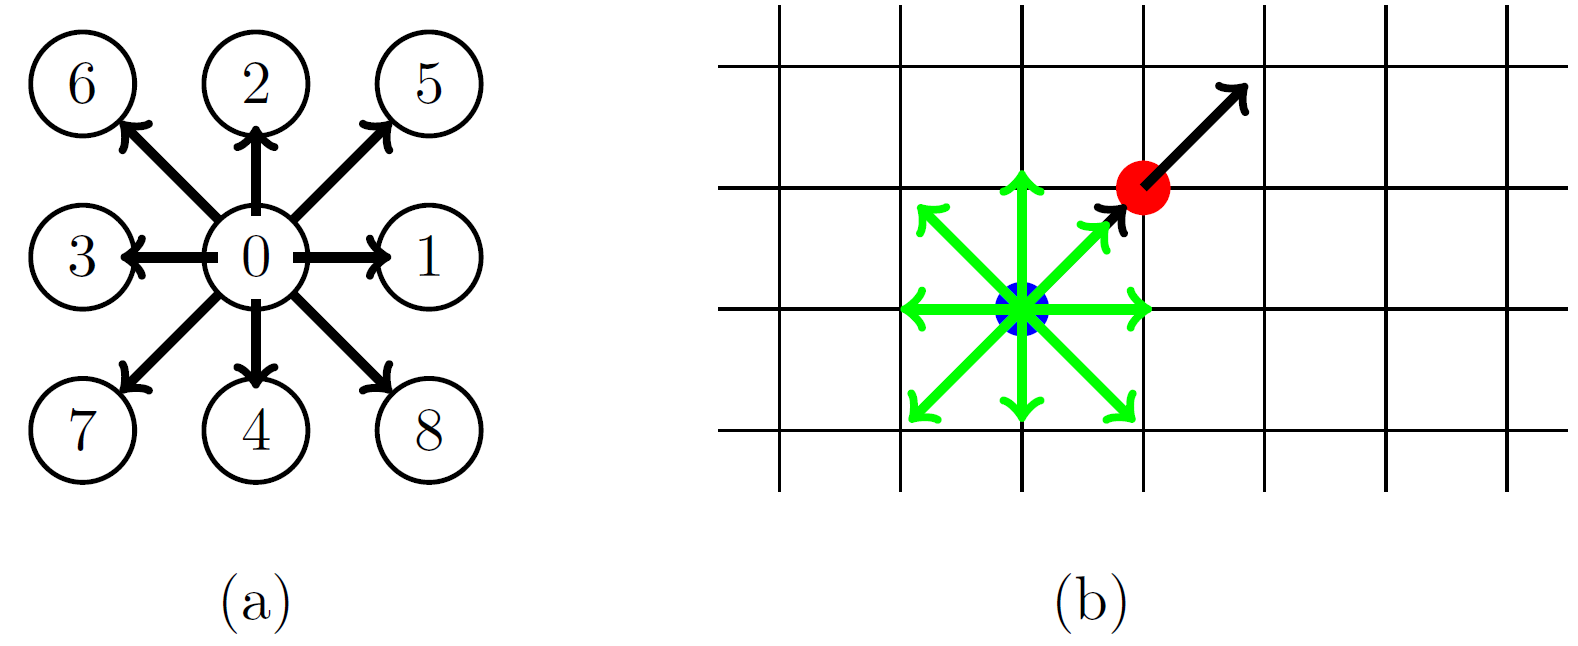
\includegraphics[width=0.4\textwidth]{logos/Gitter_LBM.png}
   \vspace{-3mm}
   \caption{
      (a) The discretization on the velocity space according to D2Q9.
      (b) The uniform two-dimensional grids for
      the discretization in the physical space.
      This figure is cited from Figure~1 in \cite{pastewka2019hpc}.
   }
  \label{fig:d2q9}
  \end{center}
  \vspace{-10mm}
\end{figure}

\section{Boundary handling}\label{boundary-handling-section}
In this section, we briefly discuss how we handle
the particles that bump into boundaries.
Note that the boundary handling is performed
after the streaming step that is discussed in the previous section
and we usually use the direction that is opposite to
the direction $i$ for the bounce-back.
For this reason, we will denote
$f^\star_i$ as the $i$-th direction
particle probability density function
after the streaming step
and $i^\star$ as the direction opposite,
i.e. {\bf reflected direction}, to $i$.
Those directions follow D2Q9 illustrated
in Figure~\ref{fig:d2q9}.
Additionally, there are the following
two ways to
implement the boundary conditions~\cite{liu2014lattice}:
\begin{enumerate}
  \item {\bf Dry nodes}:
  The boundaries are located on the link between nodes
  \item {\bf Wet nodes}:
  The boundaries are located on the lattice nodes
\end{enumerate}
Since the boundary handling will be tedious when
the boundaries are placed on the lattice nodes,
and this is the case for wet nodes,
we use {\bf dry nodes} for the implementation.

\subsection{Bounce-back from objects}\label{boundary-wall-settings}
The most basic boundary condition is 
{\bf rigid wall} or the {\bf bounce-back boundary condition}.
In this condition, we apply the process without
slip condition at the boundary.
The equation at the boundary is computed as~\cite{succi2018lattice}:
\begin{equation}
\begin{aligned}
  f_i(\xv_b, t + \dt) = f_{i^\star}^\star(\xv_b, t)
\end{aligned}
\label{discretized-rigid-wall}
\end{equation}
When the {\bf boundary moves} with the velocity of
$\Uv_w$, the variation in the moments of particles
must be taken into consideration and the equation is
modified as follows~\cite{succi2018lattice}:
\begin{equation}
  \begin{aligned}
    f_i(\xv_b, t + \dt) = f_{i^\star}^\star (\xv_b, t) - 
    2 w_i \rho_w \frac{
      \cv_i \cdot \Uv_w
    }{c_s^2}
  \end{aligned}
  \label{discretized-moving-wall}
\end{equation}
where $c_s$ is the speed of sound and 
$\rho_w$ is the density at the wall.
The computation of $\rho_w$ is usually performed by
either of the followings~\cite{zou1997pressure, khajepor2019study}:
\begin{enumerate}
  \item Take the average density $\bar{\rho}$ of the simulated field
  \item Extrapolate $\rho_w$ using 
  the particle probability density function in the physical domain by Eq~(19) in \cite{zou1997pressure}
\end{enumerate}
Although we get {\bf similar velocity fields in lid-driven cavity by both solutions},
the extrapolation is highly unstable with respect to
the wall velocity $U_w (> 0.3)$ compared to the first solution.
For this reason, we {\bf take the first solution} for this paper.
Note that we can activate the usage of the extrapolation by
{\tt --extrapolation True} from the command line as well.

\subsection{Periodic boundary conditions (PBC)}
In this section, we assume that we have
boundaries at $x = 0~(\text{inlet})$ and $X - 1~(\text{outlet})$
where $X$ is the number of the lattice grid in the $x$-axis.
The most basic PBC assumes that
the flow from outlet comes in from inlet as follows~\cite{succi2018lattice}: 
\begin{equation}
\begin{aligned}
  f(0, y, t) = f((X - 1)\dx, y, t)
\end{aligned}
\end{equation}
This condition is implicitly implemented during the streaming operation.
Another PBC handles
the pressure variation $\Delta p$ between inlet and outlet.
Since the density $\rho$ is computed as $\rho = \frac{p}{c_s^2}$
where $p$ is the pressure and $c_s$ is the speed of sound,
the density at the inlet $\rho_{\rm in} = \frac{p_{\rm in}}{c_s^2}$ and
that at the outlet $\rho_{\rm out} = \frac{p_{\rm in} + \Delta p}{c_s^2}$ can be computed
accordingly given the constant pressure $p_{\rm in}$
at the outlet.
Then the prestreaming $f^\star$ at 
the inlet and the outlet are computed as follows~\cite{succi2018lattice}:
\begin{equation}
\begin{aligned}
  f_i^\star(-\dx, y, t) &=
  f_i^{\rm eq}(\rho_{\rm in}, \uv((X - 1)\dx, y, t))
  + (f_i^\star((X - 1)\dx, y, t) - f_i^{\rm eq}((X - 1)\dx, y, t))\\
  f_i^\star(X\dx, y, t) &=
  f_i^{\rm eq}(\rho_{\rm out}, \uv(0, y, t))
  + (f_i^\star(0, y, t) - f_i^{\rm eq}(0, y, t))\\
\end{aligned}
\label{discretized-pbc-pressure}
\end{equation}
where $x = -\dx$ and $x = X\dx$ correspond to $x = (X - 1)\dx$ and $x = 0$ in this setting,
respectively.
Note that since the pressure PBC computes the prestreaming $f^\star$,
{\bf it must be performed before the streaming operation} unlike the bounce-back.


\chapter{Implementation}
\vspace{-8mm}
In this chapter, we describe how the LBM is implemented in {\tt Python}
and how to compute the LBM in parallel.
All the implementation is assuming that
the physical domain is discretized by D2Q9
and the horizontal axis is $x$ and 
the vertical axis is $y$, respectively.
Note that entire codes are based on
{\tt Numpy}~\footnote{Numpy: https://numpy.org/}
and {\tt mpi4py}~\footnote{mpi4py: https://mpi4py.readthedocs.io/en/stable/}.
Throughout the chapter, {\tt numpy} is imported as {\tt np}.

\section{Main routine}
Algorithm~\ref{alg:lattice-boltzmann-method-algorithm}
shows the pseudocode of the main processing in the LBM.
Recall that $f(\cdot, t)$.shape = $(X, Y, 9)$,
$\rho(\cdot, 0)$.shape = $(X, Y)$ and $\uv(\cdot, 0)$.shape = $(X, Y, 2)$.
First, we provide the initial values for the density and the velocity.
Then, we compute the probability function and equilibrium and
apply the collision step.
The equilibrium implementation is shown in Algorithm~\ref{alg:equilibrium-algorithm}.
After applying equilibrium, we perform the
streaming operation shown in Algorithm~\ref{alg:streaming-algorithm}
and slide each quantity to the adjacent cells.
Finally, we apply the boundary handling at each boundary cell as 
described in Algorithm~\ref{alg:boundary-conditions-algorithm}
and update the density and the velocity as in Eq~(\ref{discretized-momentum}).
Note that the order of each step might vary depending on literature~\cite{timm2016lattice, succi2018lattice}.
Since {\tt Python} slows down when using for loops
and {\tt Python} speeds up when replacing for loops with {\tt numpy} processing,
the implementations use as much slicing as possible
and high dependency on {\tt numpy} achieves 100 times speed up depending on
the settings~\cite{van2011numpy}. 

Algorithm~\ref{alg:streaming-algorithm} uses
the {\tt np.roll} operation that enables
to handle the PBC automatically.
This function rolls the array in the following manner:
\begin{equation*}
\begin{aligned}
  \text{np.roll}(f[x][y][i], \text{shift}=\cv_i, \text{axis}=(0, 1)) =
  f[nx][ny][i] \\
\end{aligned}
\end{equation*}
where
$nx = (x + \cv_i[0]) \% X, ny = (y + \cv_i[1]) \% Y$,
$i$ is the direction index in D2Q9, and $\cv_i$ is the vector
that specifies the $i$-th direction in D2Q9.
In Algorithm~\ref{alg:boundary-conditions-algorithm},
we use {\tt in\_indices} and {\tt out\_indices}
to eliminate for-loop by slicing.
Additionally, we compute $\rho_w$ as described in Section~\ref{boundary-wall-settings}.
Note that 
although the pressure PBC is included in Algorithm~\ref{alg:boundary-conditions-algorithm}
for simplicity,
only the pressure PBC updates the pre-streaming $f^\star$
and thus we need to perform it {\bf before the streaming operation}.
Additioinally, the domain is extended with virtual nodes 
at both edges of the periodic boundary in the pressure PBC
so that we can handle the boundary condition naturally. 


\begin{algorithm}[tb]
  \caption{The main routine of the lattice Boltzmann method}
  \label{alg:lattice-boltzmann-method-algorithm}
  \begin{algorithmic}[1]
    \Statex{The grid size: $X, Y$,
    Relaxation factor : $\omega$,
    Initial velocity: $\uv_0$,
    Initial density: $\rho_0$
    } \Comment{Inputs}
    \Statex{Boundary conditions}
    \Function{lattice boltzmann method}{}
    \State{$\rho(\xv, 0) = \rho_0, \uv(\xv, 0) = \uv_0$ for all $\xv \in [0, X) \times [0, Y)$}
    \For{$t= 0, 1, \dots$}
    \State{$\feq(\cdot, t)$ = equilibrium($\rho(\cdot, t), \uv(\cdot, t)$)}
    \Comment{Eq~(\ref{discretized-eq})}
    \State{$f^\star$ = $f + \omega (\feq - f)$}
    \Comment{Eq~(\ref{discretized-streaming})}
    \State{$f^\star(\cdot, t)$ =streaming($f^\star(\cdot, t)$)}
    \Comment{Eq~(\ref{discretized-streaming})}
    \State{$f(\cdot, t + 1)$ = boundary\_handling($f^\star(\cdot, t),\feq(\cdot, t)$)}
    \Comment{Eq~(\ref{discretized-rigid-wall}), (\ref{discretized-moving-wall}), (\ref{discretized-pbc-pressure})}
    \State{$\rho(\cdot, t + 1), \uv(\cdot, t + 1)$=moments\_update($f(\cdot, t + 1)$)}
    \Comment{Eq~(\ref{discretized-momentum})}
    \EndFor
    \EndFunction
  \end{algorithmic}
\end{algorithm}

\begin{algorithm}[tb]
  \caption{equilibrium}
  \label{alg:equilibrium-algorithm}
  \begin{algorithmic}[1]
    \Statex{$\wv = \text{np.array([}
    \frac{4}{9}, \frac{1}{9}, \frac{1}{9}, 
    \frac{1}{9}, \frac{1}{9}, \frac{1}{36}, 
    \frac{1}{36}, \frac{1}{36}, \frac{1}{36}
    \text{])}$, $\cv$ in Eq~(\ref{d2q9-velocity})}
    \Function{equilibrium}{$\rho$ = $\rho(\cdot, t)$, $\uv$ = $\uv(\cdot, t)$}
    \Comment{$\uv$.shape = $(X, Y, 2)$, $\rho$.shape = $(X, Y)$}
    \State{u\_norm2 = ($\uv$ ** 2).sum(axis=-1)[..., None]}
    \State{u\_at\_c = $\uv$ @ $\cv^\top$}
    \Comment{u\_at\_c.shape = $(X, Y, 9)$}
    \State{w\_tmp, $\rho$\_{tmp} = $\wv$[None, None, ...], $\rho$[..., None]}
    \Comment{Adapt the shapes to u\_at\_c}
    \State{$\feq$ = w\_tmp * $\rho$\_tmp * (1 + 3 * u\_at\_c + 4.5 * (u\_at\_c) ** 2)-1.5 * u\_norm2}
    \State{{\bf return} $\feq$}
    \EndFunction
  \end{algorithmic}
\end{algorithm}

\begin{algorithm}[tb]
  \caption{Streaming operation}
  \label{alg:streaming-algorithm}
  \begin{algorithmic}[1]
    \Statex{$\cv$ in Eq~(\ref{d2q9-velocity})}
    \Function{streaming}{$f^\star$ = $f^\star(\cdot, t)$}
    \State{$f^{\rm post}$ = np.zeros\_like($f^\star$)}
    \For{$i= 0, 1, \dots, 8$}
    \State{$f^{\rm post}[..., i]$=np.roll($f^\star$[..., i], shift=$\cv_i$, axis=(0, 1))}
    \Comment{Slide $f^\star$ one step to c[i]}
    \EndFor
    \State{{\bf return} $f^{\rm post}$}
    \EndFunction
  \end{algorithmic}
\end{algorithm}

\begin{algorithm}[t]
  \caption{Boundary conditions (Pressure PBC is also included for simplicity)}
  \label{alg:boundary-conditions-algorithm}
  \begin{algorithmic}[1]
    \Statex{
      The indices in D2Q9 s.t. the flow comes in
      given boundaries: in\_indices
    }
    \Statex{
      The indices in D2Q9 s.t. the flow goes out
      given boundaries: out\_indices
    }
    \Function{boundary handlling}{$f^\star$ = $f^\star(\cdot, t)$,
      $\feq$ = $\feq(\cdot, t)$}
    \If{Pressure PBC}
    \Comment{fluid flows from $x = 0$ to $X - 1$}
    \State{{\bf \# Note: Pressure PBC must be applied before streaming operation}}
    \State{$\feq_{\rm in}, \feq_{\rm out}$ = equilibrium($\rho_{\rm in}$, $\uv$[-2]), equilibrium($\rho_{\rm out}$, $\uv$[1])}
    \State{$f^\star$[0, :,out\_indices]=$\feq_{\rm in}$[:,out\_indices].T+($f^\star$[-2, :,out\_indices]-$\feq$[-2, :,out\_indices])}
    \State{$f^\star$[-1, :,in\_indices]=$\feq_{\rm out}$[:,in\_indices].T+($f^\star$[1, :,in\_indices] - $\feq$[1, :,in\_indices])}
    \EndIf
    \If{Rigid wall}
    \Comment{The case when the wall is at the top}
    \State{$f$[:, -1, in\_indices] = $f^\star$[:, -1, out\_indices]}
    \EndIf
    \If{Moving wall}
    \Comment{The case when the wall is at the top}
    \State{coef = np.zeros\_like((X, Y, 9))}
    \State{value = 2 * $\wv$[out\_indices] * ($\cv$[out\_indices] @ $\uv$) / $c_s$ ** 2}
    \State{coef[:, -1, out\_indices] = value[np.newaxis, :]}
    \State{$f$[:, -1, in\_indices] = $f^\star$[:, -1, out\_indices] $- \rho_w$ * coef[:, -1, out\_indices]}
    \EndIf
    \State{{\bf return} $f$}
    \EndFunction
  \end{algorithmic}
\end{algorithm}

\section{Parallel computation by MPI}\label{section-mpi}
In order to process the LBM in parallel,
we employ the spatial domain decomposition and
the messaging passing interface (MPI)
so that we can compute the collision step of the LBM
in parallel.
This is possible because the collision step does not require
any communication between processes~\cite{pastewka2019hpc}.
Then, we explain how we divide the domain.
Suppose we are provided the number of processes of $P$,
we first factorize $P$ such that $P = P_x \times P_y$
where $P_x, P_y \in \mathbb{Z}^{+}$,
$P_x, P_y = \text{arg} \min_{P_x, P_y}(|| P_y - P_x ||)$
and $P_x \leq P_y$ if $X \leq Y$ otherwise $P_y \leq P_x$.
Then, we divide the $x$-axis into $P_x$ intervals and
the $y$-axis into $P_y$ intervals where
any pairs of intervals $I_{i}, I_{j}$ in the same direction satisfy
$-1 \leq || I_{i} || - ||I_{j}|| \leq 1$.
Note that $||I||$ is the size of the interval $I$.
This split of the domain achieves the most balanced distribution of
the computation.
For the streaming step, we need to consider particles
moving from one process to another.
We implement it using so-called {\bf ghost cells}
around the actual computational domain.
Figure~\ref{mpi-conceptual} shows the conceptual visualization of
how each process communicates and ghost cells work.
Since each process requires the four edges of adjacent
processes, the communications are required four times
for each process.
Algorithm~\ref{alg:mpi-algorithm}
shows the implementation using {\tt mpi4py}.
{\tt grid\_manager} is the self-developed module
that manages useful information related to
the process location, the adjacent relation, and so on.
{\tt Sendrecv} function is used for the communication and
each process receives an array from {\tt dest} that is sent
by {\tt neighbor} and sends an array {\tt sendbuf} to
{\tt neighbor}.
Note that {\tt buf} is the abbreviation of buffer and
used for the buffer to communicate data.

\begin{figure}
  \centering
  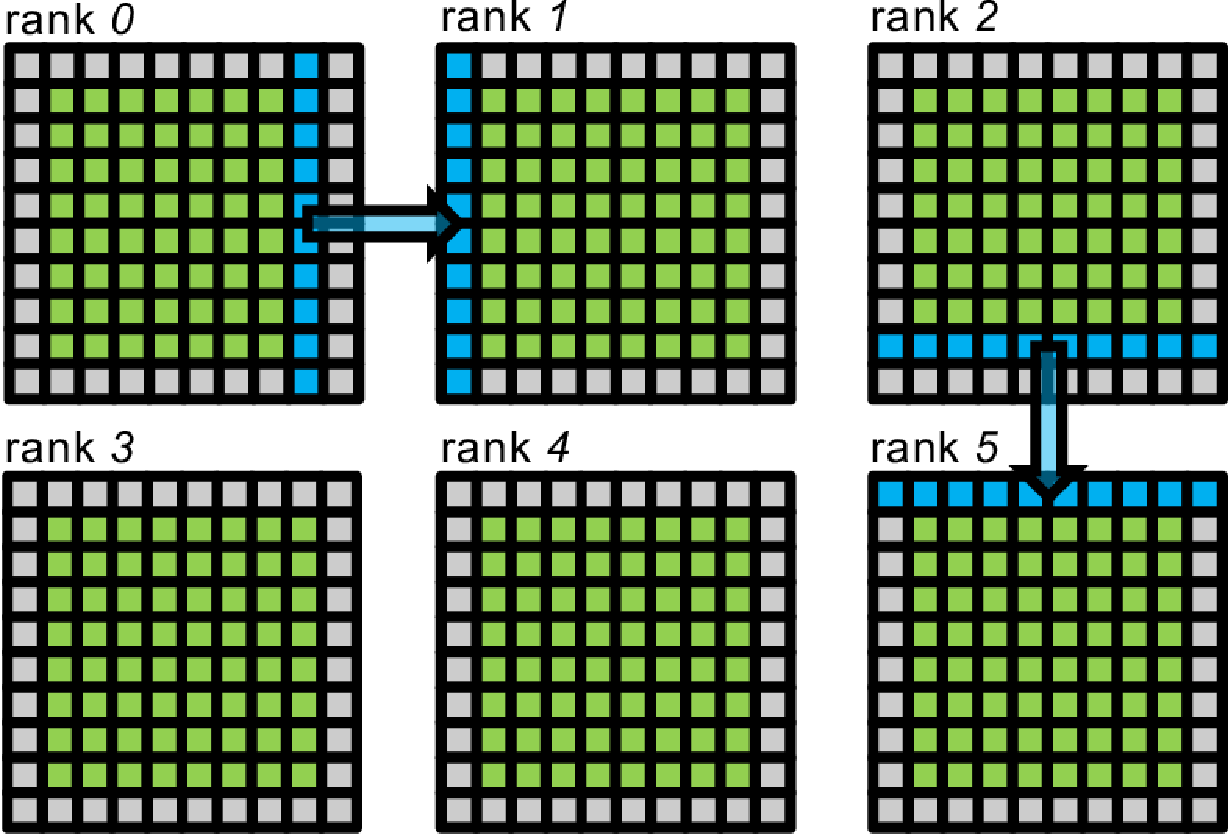
\includegraphics[width=0.48\textwidth]{imgs/mpi-conceptual.pdf}
  \caption{
    Domain decomposition and communication strategy in MPI.
    As described in the main text, we first divide each axis
    into $P_x$ and $P_y$ intervals and divide by the intervals.
    Each rank has green lattice points and this area is the active physical domain.
    Then we add additional ghost cells for buffer (gray lattice points).
    During each communication step, the outermost green active lattice
    sends the data to the adjacent outermost ghost lattice (blue arrows).
    The figure is cited from Figure~2 in ~\cite{pastewka2019hpc}.
  }
  \label{mpi-conceptual}
\end{figure}

\begin{algorithm}[b]
  \caption{The communication of
  the particle probability density function}
  \label{alg:mpi-algorithm}
  \begin{algorithmic}[1]
    \Statex{Process and lattice grids management: grid\_manager}
    \Function{communication}{}
    \State{{\bf for} dir in grid\_manager.neighbor\_directions {\bf do}}
    \Comment{Iterate over the D2Q9 index}
    \Indent
    \State{dx, dy = $\cv_i$}
    \State{sendidx = grid\_manager.step\_to\_idx(dx, dy, send=True)}
    \State{recvidx = grid\_manager.step\_to\_idx(dx, dy, send=False)}
    \State{neighbor = grid\_manager.get\_neighbor\_rank(dir)}
    \If{dx == 0} \Comment{send to top and bottom}
    \State{sendbuf = $f$[:, sendidx, ...].copy()}
    \State{grid\_manager.rank\_grid.Sendrecv(sendbuf=sendbuf, dest=neighbor,}
    \State{\hspace{56mm} recvbuf=recvbuf, source=neighbor)}
    \State{$f$[:, recvidx, ...] = recvbuf}
    \ElsIf{dy == 0} \Comment{send to left and right}
    \State{sendbuf = $f$[sendidx, ...].copy()}
    \State{grid\_manager.rank\_grid.Sendrecv(sendbuf=sendbuf, dest=neighbor,}
    \State{\hspace{56mm} recvbuf=recvbuf, source=neighbor)}
    \State{$f$[recvidx, ...] = recvbuf}
    \EndIf
    \EndIndent
    \State{{\bf return} $f$}
    \EndFunction
  \end{algorithmic}
\end{algorithm}

\section{Software quality}
All the codes follow {\tt pep8 style}~\footnote{https://www.python.org/dev/peps/pep-0008/}
and {\tt Google Python Style documentation string}~\footnote{https://google.github.io/styleguide/pyguide.html}.
In order to make the codes robust to unexpected errors,
we introduce
{\tt Flake8}~\footnote{https://flake8.pycqa.org/en/latest/}
and {\tt MyPy} static typing check~\footnote{http://mypy-lang.org/} as well.
Furthermore, all the components are tested by
{\tt unittest}\footnote{https://docs.python.org/3/library/unittest.html}
and we provide {\tt requirements.txt}
and the shell scripts for the main experiments
to reproduce the complete running conditions.
Those tools {\bf guarantee the reproducibility} of the experiments.
Furthermore, the implementations focus on abstraction and
most codes are abstracted to reduce the coding lines as much as possible.
Therefore, the codes are {\bf highly reusable} and
the implementation has only one explicit coding for
each Algorithm provided in this chapter.
Furthermore, {\tt ArgumentParser} allows users to
pass an arbitrary setting to run the experiments
and it {\bf contributes to the generality} in this code.
All the instructions are available at {\tt Github} repository
described in Chapter~1.


\chapter{Numerical results}
\vspace{-8mm}
In the previous chapter, we discuss the implementation details
and how we apply the LBM to various settings.
In this chapter, we first illustrate
how to validate the implementations and 
then show the visualizations and numerical results
obtained from the series experiments.

\section{Validation experiments}
In the physics simulation, it is always important
to validate whether the implementations are correct.
Therefore, we first show how to validate the implementation
using several examples.

\subsection{Shear wave decay}
The shear wave decay represents the time evolution of a
velocity perturbation in the flow.
Since the viscosity decays the velocity of the flow,
the velocity converges to zero in the end.
When we set the following sinusoidal perturbation in the velocity
as the initial condition:
\begin{equation}
  \begin{aligned}
    \uv(\xv, t = 0) =
    \begin{bmatrix}
      u_x(y, t = 0) \\
      0 \\
    \end{bmatrix}
    =  
    \begin{bmatrix}
      \epsilon \sin \frac{2\pi y}{Y} \\
        0 \\
      \end{bmatrix}
  \end{aligned}.
  \label{shear-vel-init}
\end{equation}
Then the analytical solution for the time evolution of 
the velocity is calculated as follows~\cite{fei2018three}:
\begin{equation}
  \begin{aligned}
    u_x(y, t) &= 
    \epsilon \exp\biggl(
      -\nu \biggl(
        \frac{2\pi}{Y}
      \biggr)^2 t\biggr) \sin \frac{2\pi y}{Y}.
  \end{aligned}
  \label{sinusoidal-vel-analytical-solution}
\end{equation}
Note that this result is obtained using Navier-Stokes equations for incompressible fluid
and the assumptions that the pressure term $\nabla p$ and
the convection term $(\uv \cdot \nabla) \uv$ are negligible 
compared to the viscosity term $\nu \nabla^2 \uv$.
In Figure~\ref{fig:sinusoidal-velocity}, we show the plot of both
simulated results and the analytical solution of sinusoidal velocity.
Note that the initial condition follows Eq.~(\ref{shear-vel-init}). 
As seen in the figure, the simulated results and the analytical solution
{\bf perfectly fit} and thus we could validate our implementation of
rigid wall and moments updates.
Figure~\ref{fig:sinusoidal-density} shows the density distribution
over time.
This simulation uses the sinusoidal density in the $x$-direction
\begin{equation}
\begin{aligned}
  \rho(\xv, 0) = \rho_{\rm b} + \epsilon \sin \frac{2 \pi x}{X}.
\end{aligned}
\label{sinusoidal-density-init}
\end{equation}
where $\rho_{\rm b}$ is a positive constant value.
As seen in the figure, the sinusoidal density also
yields the convergence.
On the other hand, the sinusoidal density has
a swing of the maxima and the minima unlike the sinusoidal velocity.

\begin{figure}[H]
  \begin{center}
    \subfloat[$t = 0$]{
      \includegraphics[width=0.23\textwidth]{../log/sinusoidal_velocity/fig/vel000000.pdf}
    }
    \subfloat[$t = 150$]{
      \includegraphics[width=0.23\textwidth]{../log/sinusoidal_velocity/fig/vel000150.pdf}
    }
    \subfloat[$t = 300$]{
      \includegraphics[width=0.23\textwidth]{../log/sinusoidal_velocity/fig/vel000300.pdf}
    }
    \subfloat[$t = 450$]{
      \includegraphics[width=0.23\textwidth]{../log/sinusoidal_velocity/fig/vel000450.pdf}
    }\\
    \vspace{-3mm}
    \subfloat[$t = 600$]{
      \includegraphics[width=0.23\textwidth]{../log/sinusoidal_velocity/fig/vel000600.pdf}
    }
    \subfloat[$t = 750$]{
      \includegraphics[width=0.23\textwidth]{../log/sinusoidal_velocity/fig/vel000750.pdf}
    }
    \subfloat[$t = 900$]{
      \includegraphics[width=0.23\textwidth]{../log/sinusoidal_velocity/fig/vel000900.pdf}
    }
    \subfloat[$t = 1050$]{
      \includegraphics[width=0.23\textwidth]{../log/sinusoidal_velocity/fig/vel001050.pdf}
    }\\
    \vspace{-3mm}
    \subfloat[Time evolution of velocity at $y = {\rm arg}\max_{y^\prime} u_x(y^\prime, t=0)$]{
      \includegraphics[width=0.77\textwidth]{../log/sinusoidal_velocity/fig/vel_time_evolution.pdf}
    }
    % \vspace{-3mm}
    % \subfloat[$t = 1200$]{
    %   \includegraphics[width=0.23\textwidth]{../log/sinusoidal_velocity/fig/vel001200.pdf}
    % }
    % \subfloat[$t = 1350$]{
    %   \includegraphics[width=0.23\textwidth]{../log/sinusoidal_velocity/fig/vel001350.pdf}
    % }
    % \subfloat[$t = 1500$]{
    %   \includegraphics[width=0.23\textwidth]{../log/sinusoidal_velocity/fig/vel001500.pdf}
    % }
    % \subfloat[$t = 1650$]{
    %   \includegraphics[width=0.23\textwidth]{../log/sinusoidal_velocity/fig/vel001650.pdf}
    % }\\
    \caption{
      The time evolution of the sinusoidal velocity
      in Eq.~(\ref{shear-vel-init}) at
      the $x = 25$ in the lattice grid size of $(50, 50)$.
      The $x$-axis shows the location in the $y$ direction
      and the $y$-axis shows the magnitude of velocity at 
      the corresponding location.
      The coefficients $\epsilon$ in Eq.~(\ref{shear-vel-init}) and
      the initial density $\rho_0$
      are set to $0.01$ and $1.0$ respectively.
      The relaxation term $\omega$ is set to $1.0$.
      \label{fig:sinusoidal-velocity}}
  \end{center}
\end{figure}

As discussed, moment fluctuations decay exponentially and
such a decay is represented as follows~\cite{palmer1994transverse, hess2002determining}:
\begin{equation}
  \begin{aligned}
    Q_t(t) &= \exp\biggl(
      -\nu \biggl(
        \frac{2\pi}{X}
      \biggr)^2 t\biggr)
  \end{aligned}
  \label{viscosity-analytical}
\end{equation}
where $Q(\xv, t) = \epsilon Q_x(\xv) Q_t(t)$
and $Q(\xv, t)$ is one of the moment quantities.
Note that we assume that the assumptions for Eq.~(\ref{sinusoidal-vel-analytical-solution}) hold
and the case of the sinusoidal velocity is equivalent to Eq.~(\ref{sinusoidal-vel-analytical-solution})~\cite{fei2018three}.
We perform the experiments to validate the implementation via the viscosity estimated by Eq.~(\ref{viscosity-analytical}) using
the exact experiment settings for Figure~\ref{fig:sinusoidal-velocity}
and Figure~\ref{fig:sinusoidal-density}
except the relaxation term $\omega$.
The analytical viscosity is computed as $\nu = c_{\rm s}^2 (\frac{1}{\omega} - \frac{1}{2})$~\cite{timm2016lattice}.
For the experiments, the simulated viscosity is computed based on the exponential decay curve, i.e. Eq.~(\ref{viscosity-analytical}),
of the density and velocity using 
{\tt curve\_fit}~\footnote{https://docs.scipy.org/doc/scipy/reference/generated/scipy.optimize.curve\_fit.html}.
{\tt curve\_fit} approximates the optimal viscosity $\nu$ from the observations.
Since the densities swing so much and a smooth exponential decay curve
is not obtained, we only take the maximum of the swinging.
Such time-series data is obtained by
{\tt argrelextrema}~\footnote{https://docs.scipy.org/doc/scipy/reference/generated/scipy.signal.argrelextrema.html}.
The results are shown in Figure~\ref{fig:omega-vs-visc}.
Based on the results, $\omega$ close to $0.0$ and $2.0$
leads to numerical instability.
Otherwise, the simulated results and analytical solution fit perfectly.
Therefore, we need to avoid using $\omega$ closer to $0$ or $2$ for more accurate results.

\begin{figure}[H]
  \begin{center}
    \subfloat[$t = 0$]{
      \includegraphics[width=0.23\textwidth]{../log/sinusoidal_density/fig/density000000.pdf}
    }
    \subfloat[$t = 150$]{
      \includegraphics[width=0.23\textwidth]{../log/sinusoidal_density/fig/density000150.pdf}
    }
    \subfloat[$t = 300$]{
      \includegraphics[width=0.23\textwidth]{../log/sinusoidal_density/fig/density000300.pdf}
    }
    \subfloat[$t = 450$]{
      \includegraphics[width=0.23\textwidth]{../log/sinusoidal_density/fig/density000450.pdf}
    }\\
    \vspace{-3mm}
    \subfloat[$t = 600$]{
      \includegraphics[width=0.23\textwidth]{../log/sinusoidal_density/fig/density000600.pdf}
    }
    \subfloat[$t = 750$]{
      \includegraphics[width=0.23\textwidth]{../log/sinusoidal_density/fig/density000750.pdf}
    }
    \subfloat[$t = 900$]{
      \includegraphics[width=0.23\textwidth]{../log/sinusoidal_density/fig/density000900.pdf}
    }
    \subfloat[$t = 1050$]{
      \includegraphics[width=0.23\textwidth]{../log/sinusoidal_density/fig/density001050.pdf}
    }\\
    \vspace{-3mm}
    \subfloat[Time evolution of density at $x = {\rm arg}\max_{x^\prime} \rho(x^\prime, t=0)$]{
      \includegraphics[width=0.77\textwidth]{../log/sinusoidal_density/fig/density_time_evolution.pdf}
    }
    % \vspace{-3mm}
    % \subfloat[$t = 1200$]{
    %   \includegraphics[width=0.23\textwidth]{../log/sinusoidal_density/fig/density001200.pdf}
    % }
    % \subfloat[$t = 1350$]{
    %   \includegraphics[width=0.23\textwidth]{../log/sinusoidal_density/fig/density001350.pdf}
    % }
    % \subfloat[$t = 1500$]{
    %   \includegraphics[width=0.23\textwidth]{../log/sinusoidal_density/fig/density001500.pdf}
    % }
    % \subfloat[$t = 1650$]{
    %   \includegraphics[width=0.23\textwidth]{../log/sinusoidal_density/fig/density001650.pdf}
    % }\\
    \caption{The time evolution of the sinusoidal density
    in Eq.~(\ref{sinusoidal-density-init})
      at $y = 25$ in the lattice grid size of $(50, 50)$.
      The $x$-axis shows the location in the $x$ direction
      and the $y$-axis shows the magnitude of density.
      The coefficients $\epsilon$ and $\rho_{\rm b}$ in Eq.~(\ref{sinusoidal-density-init})
      are set to $0.01$ and $1.0$ and the velocity is initialized by
      $\uv(\xv, 0) = (0,0)$.
      The relaxation term $\omega$ is set to $1.0$.
      \label{fig:sinusoidal-density}}
  \end{center}
\end{figure}

\begin{figure}[H]
  \begin{center}
    \subfloat[Sinusoidal density]{
      \includegraphics[width=0.46\textwidth]{../log/sinusoidal_velocity/fig/omega_vs_visc.pdf}
    }
    \subfloat[Sinusoidal velocity]{
      \includegraphics[width=0.46\textwidth]{../log/sinusoidal_density/fig/omega_vs_visc.pdf}
    }
    \caption{The simulated viscosity value 
    over various relaxation values $\omega$.
    The analytical solution uses $\nu = c_{\rm s}^2(\frac{1}{\omega} - \frac{1}{2})$
    and the simulated viscosity $\nu$ is approximated from an exponential decay curve in Eq.~(\ref{viscosity-analytical}).
    The simulation is performed $T = 3000$ steps
    and we take the maximum magnitude of
    $\| u_x \|$ for (a) and $\| \rho - \rho_{\rm b} \|$ for (b)
    to fit the curve.
    Note that (a) uses the same parameters as in 
    Figure~\ref{fig:sinusoidal-velocity}
    and (b) uses the same parameters as in
    Figure~\ref{fig:sinusoidal-density}.
    \label{fig:omega-vs-visc}}
  \end{center}
\end{figure}

\begin{figure}[H]
  \centering
  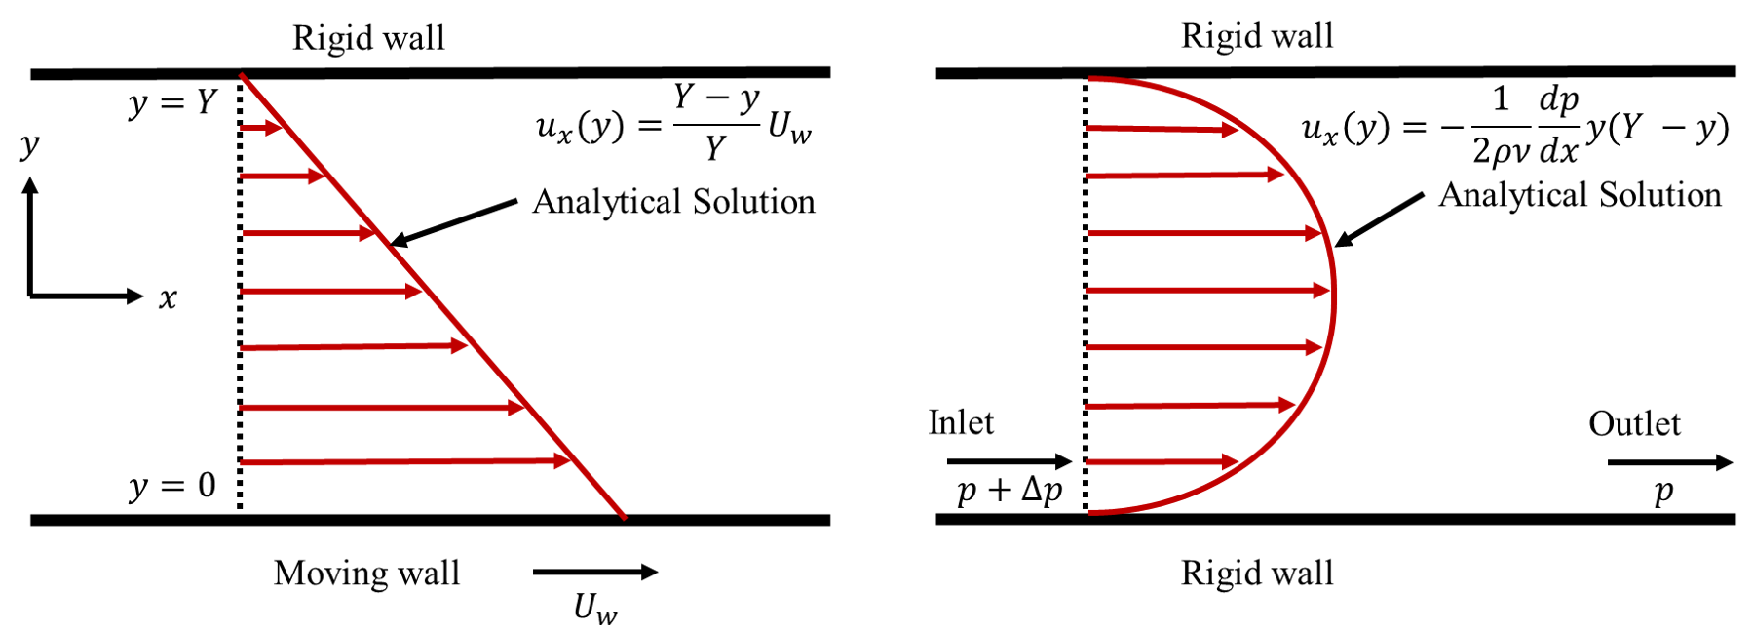
\includegraphics[width=0.98\textwidth]{imgs/couette_and_poiseuille.pdf}
  \vspace{-3mm}
  \caption{The conceptual visualizations of the Couette flow (Left) and
  Poiseuille flow (Right).}
  \vspace{-3mm}
  \label{couette-and-poiseuille-conceptual}
\end{figure}


\subsection{Couette flow}
The Couette flow is the flow between two walls as shown in
Figure~\ref{couette-and-poiseuille-conceptual}:
One is fixed and the other moves horizontally with the velocity of $U_{\rm w}$.
The flow is caused by the viscous drag force acting on the fluid.
Since the Couette flow also has an analytical solution,
we can validate the implementation of the moving wall.
The analytical solution for Figure~\ref{couette-and-poiseuille-conceptual} is given by
\begin{equation*}
\begin{aligned}
  u_x(\cdot, y) =\frac{Y - y}{Y}U_{\rm w}
\end{aligned}
\end{equation*}
~\cite{nagy2019graphical} where $Y$ is the distance between the two walls
and $u_x(\cdot, y)$ is the horizontal velocity of the flow
given a position $(x, y)$.
Note that $u_x(\cdot, y)$ does not depend on $x$.
In the experiment, we apply the bounce-back boundary condition
at the moving wall and the rigid wall
and the PBC at the inlet and outlet.
As shown in Figure~\ref{fig:couette-velocity-evolution},
the flow velocity iteratively approaches
the analytical solution and it perfectly fits in the end
and {\bf the velocity stops growing} at the time step of $t = 6000 \sim 10000$.
This experiment validates the moving wall implementation.

\begin{figure}[H]
  \vspace{-1mm}
  \centering
  \includegraphics[width=0.90\textwidth]{../log/couette_flow/fig/couette_flow_joint.pdf}
  \vspace{-5mm}
  \caption{The velocity evolution of every $500$ time steps at
  $x = 25$ in the lattice grid size of $(50, 50)$ until the time step of $t = 10000$.
  The wall velocity $U_{\rm w}$ at the bottom and the relaxation term $\omega$ are set
  to $0.1$ and $1.0$ respectively.
  We use {\bf dry node} as described in Section~\ref{boundary-handling-section}
  and the computation of wall density follows Section~\ref{boundary-wall-settings}.
  The initial density and velocity are $\rho(\xv) = 1.0, \uv(\xv) = (0, 0)$.
  \label{fig:couette-velocity-evolution}}
\end{figure}

\subsection{Poiseuille flow}
The Poiseuille flow is the flow between two non-moving walls as shown in Figure~\ref{couette-and-poiseuille-conceptual}.
The flow is caused by a constant pressure difference $\od{p}{x}$
in the horizontal direction of the two walls.
The Poiseuille flow also has the analytical solution
and we can validate the implementation of the pressure PBC.
The analytical solution for Figure~\ref{couette-and-poiseuille-conceptual} is given by
\begin{equation*}
\begin{aligned}
  u_x(\cdot, y) = - \frac{1}{2\bar{\rho} \nu} \od{p}{x} y (Y - y)
\end{aligned}
\end{equation*}
~\cite{mendiburu2009analytical}
where $\bar{\rho}$ is the average density.
In the experiment, we apply the bounce-back boundary condition
at the moving wall and the rigid wall
and the pressure PBC at the inlet and outlet.
Figure~\ref{fig:poiseuille-velocity-evolution} presents the results
and the simulated results approach the analytical solution.
In the end, it fits completely
and {\bf the velocity stops growing} at the time step of $t = 7000 \sim 10000$.

\begin{figure}[H]
  \vspace{-3mm}
  \centering
  \includegraphics[width=0.90\textwidth]{../log/poiseuille_flow/fig/poiseuille_flow_joint.pdf}
  \vspace{-3mm}
  \caption{The velocity evolution of every $500$ time steps at
  $x = 25$ in the lattice grid size of $(50, 50)$ until the time step of $t = 10000$.
  The relaxation term $\omega$ is set to $1.0$.
  The density at the inlet $\rho_{\rm in}$ and the density
  at the outlet $\rho_{\rm out}$ are set to $1.005$ and $1.0$ respectively.
  Then $\od{p}{x}$ is computed by $c_{\rm s}^2(\rho_{\rm out} - \rho_{\rm in}) / X$.
  The initial density and velocity are $\rho(\xv) = 1.0, \uv(\xv) = (0, 0)$.
  \label{fig:poiseuille-velocity-evolution}}
\end{figure}

\section{Lid-driven cavity}
Finally, we handle a concrete example.
In this paper, the lid-driven cavity shown in Figure~\ref{lid-driven-cavity-conceptual} is simulated.
The lid-driven cavity simulates the flow inside a box with
three rigid walls and one moving wall, i.e. a lid.
In this simulation, the turbulence is caused 
when the following Reynolds number is larger than 1000~\cite{chiang1998effect}:
\begin{equation*}
\begin{aligned}
  \text{Re} = \frac{LU}{\nu}
\end{aligned}
\end{equation*}
where $L$ is the characteristic length parameter
of the body and $U$ is the stream flow velocity.
One key property of the Reynolds number is that two flow system
is dynamically similar if the Reynolds number and the geometry are similar~\cite{kundu2008fluid}.
Therefore, we present the results with various 
viscosity $\nu$ and the wall velocity $U = U_{\rm w}$ that 
satisfy the Reynolds number of $1000$ under $L = X = Y = 300$
in Figure~\ref{fig:sliding-lid-reynolds-comparison}.
In the figures, all the settings converge to a similar flow in the end
as indicated in the key property of the Reynolds number.
Figure~\ref{fig:sliding-lid-velocity-evolution} shows the time evolution of
the streaming plot with the Reynolds number of $1000$.
The series of figure shows that the streaming changes gradually
and starts to have spirals at a corner due to the turbulence.
{\bf The time evolution of the velocity streaming plot is provided in
Github}~\footnote{https://github.com/nabenabe0928/high-performance-computing-fluid-dynamics-with-python/}.
Note that all the experiments for
Figure~\ref{fig:sliding-lid-reynolds-comparison}, \ref{fig:sliding-lid-velocity-evolution}
are {\bf performed using MPI of 9 processes}
and Table~\ref{tab:parallel-validation}
shows the validation of the parallel implementation.
Since the summation of the absolute error of the velocity over the whole domain
is $0.0$, it is obvious that
{\bf the parallel implementation behaves identically to the serial implementation}.
The test code for an arbitrary setting is available at {\tt run\_scripts/compare\_parallel\_vs\_serial.sh}
in the repository.

\begin{figure}[t]
  \vspace{-7mm}
  \centering
  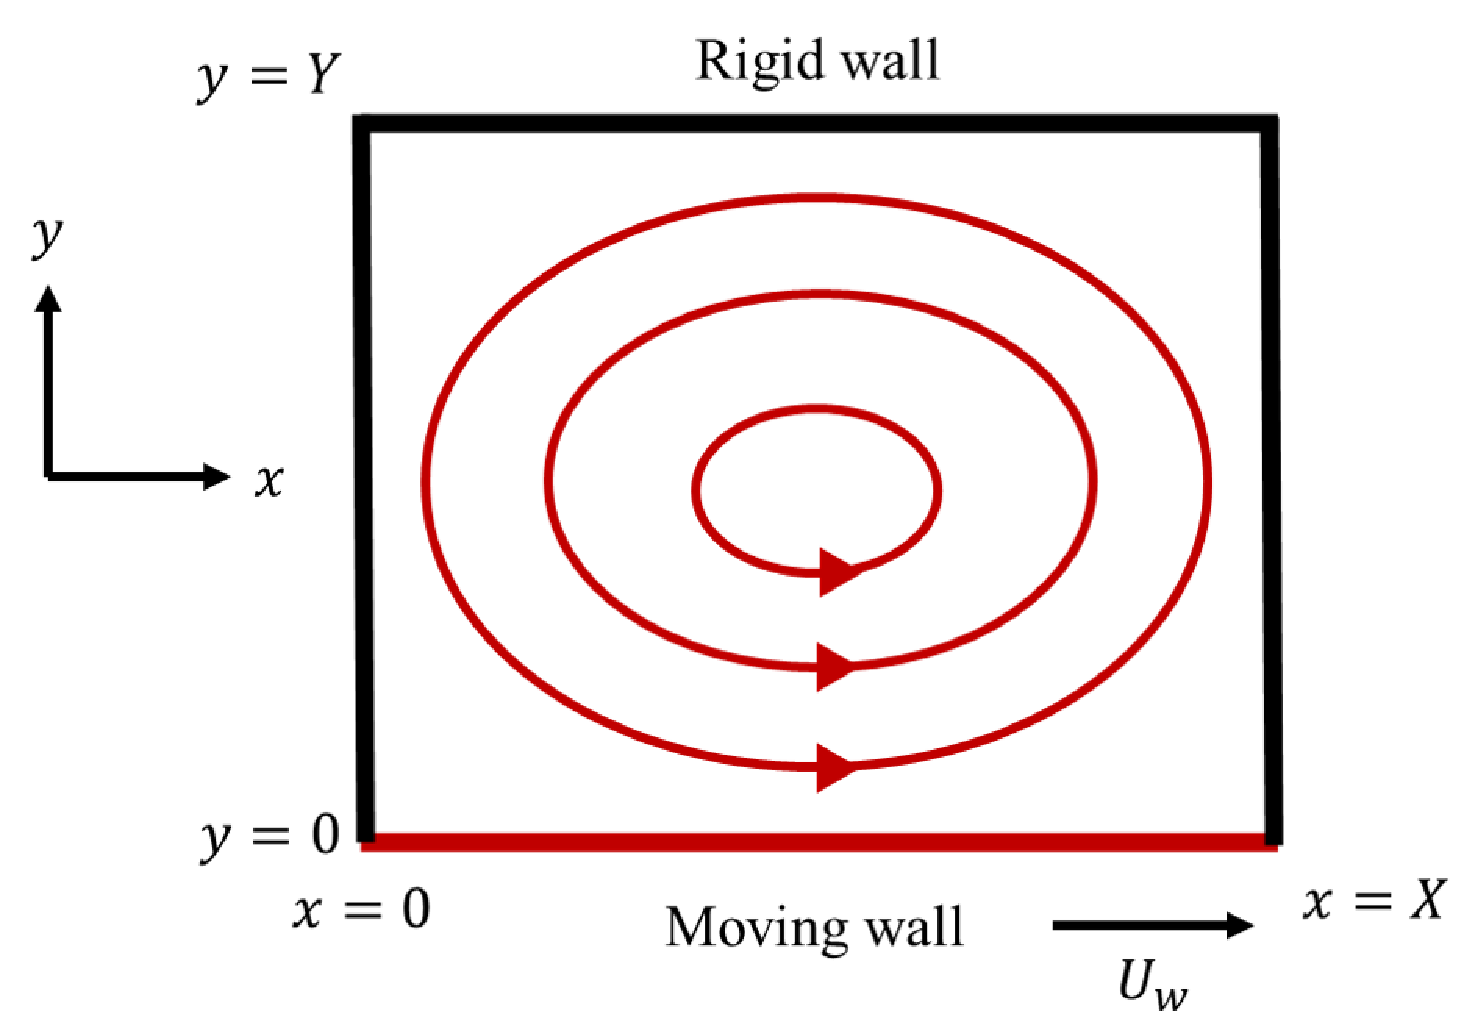
\includegraphics[width=0.48\textwidth]{imgs/lid-driven-cavity.pdf}
  \vspace{-5mm}
  \caption{The conceptual visualizations of the lid-driven cavity.}
  \label{lid-driven-cavity-conceptual}
  \vspace{-3mm}
\end{figure}

\begin{figure}[t]
  \begin{center}
    \subfloat[$U_{\rm w} = 0.1, \nu = 0.03$]{
      \includegraphics[width=0.24\textwidth]{../log/sliding_lid_W0.10_visc0.03_size75x75_parallel/fig/vel_flow100000.pdf}
    }
    \subfloat[$U_{\rm w} = 0.2, \nu = 0.06$]{
      \includegraphics[width=0.24\textwidth]{../log/sliding_lid_W0.20_visc0.06_size75x75_parallel/fig/vel_flow100000.pdf}
    }
    \subfloat[$U_{\rm w} = 0.3, \nu = 0.09$]{
      \includegraphics[width=0.24\textwidth]{../log/sliding_lid_W0.30_visc0.09_size75x75_parallel/fig/vel_flow100000.pdf}
    }
    \subfloat[$U_{\rm w} = 0.4, \nu = 0.12$]{
      \includegraphics[width=0.24\textwidth]{../log/sliding_lid_W0.40_visc0.12_size75x75_parallel/fig/vel_flow100000.pdf}
    }\\
    \subfloat[$U_{\rm w} = 0.1, \nu = 0.03$]{
      \includegraphics[width=0.24\textwidth]{../log/sliding_lid_W0.10_visc0.03_size150x150_parallel/fig/vel_flow100000.pdf}
    }
    \subfloat[$U_{\rm w} = 0.2, \nu = 0.06$]{
      \includegraphics[width=0.24\textwidth]{../log/sliding_lid_W0.20_visc0.06_size150x150_parallel/fig/vel_flow100000.pdf}
    }
    \subfloat[$U_{\rm w} = 0.3, \nu = 0.09$]{
      \includegraphics[width=0.24\textwidth]{../log/sliding_lid_W0.30_visc0.09_size150x150_parallel/fig/vel_flow100000.pdf}
    }
    \subfloat[$U_{\rm w} = 0.4, \nu = 0.12$]{
      \includegraphics[width=0.24\textwidth]{../log/sliding_lid_W0.40_visc0.12_size150x150_parallel/fig/vel_flow100000.pdf}
    }\\
    \subfloat[$U_{\rm w} = 0.1, \nu = 0.03$]{
      \includegraphics[width=0.24\textwidth]{../log/sliding_lid_W0.10_visc0.03_size225x225_parallel/fig/vel_flow100000.pdf}
    }
    \subfloat[$U_{\rm w} = 0.2, \nu = 0.06$]{
      \includegraphics[width=0.24\textwidth]{../log/sliding_lid_W0.20_visc0.06_size225x225_parallel/fig/vel_flow100000.pdf}
    }
    \subfloat[$U_{\rm w} = 0.3, \nu = 0.09$]{
      \includegraphics[width=0.24\textwidth]{../log/sliding_lid_W0.30_visc0.09_size225x225_parallel/fig/vel_flow100000.pdf}
    }
    \subfloat[$U_{\rm w} = 0.4, \nu = 0.12$]{
      \includegraphics[width=0.24\textwidth]{../log/sliding_lid_W0.40_visc0.12_size225x225_parallel/fig/vel_flow100000.pdf}
    }\\
    \subfloat[$U_{\rm w} = 0.1, \nu = 0.03$]{
      \includegraphics[width=0.24\textwidth]{../log/sliding_lid_W0.10_visc0.03_size300x300_parallel/fig/vel_flow100000.pdf}
    }
    \subfloat[$U_{\rm w} = 0.2, \nu = 0.06$]{
      \includegraphics[width=0.24\textwidth]{../log/sliding_lid_W0.20_visc0.06_size300x300_parallel/fig/vel_flow100000.pdf}
    }
    \subfloat[$U_{\rm w} = 0.3, \nu = 0.09$]{
      \includegraphics[width=0.24\textwidth]{../log/sliding_lid_W0.30_visc0.09_size300x300_parallel/fig/vel_flow100000.pdf}
    }
    \subfloat[$U_{\rm w} = 0.4, \nu = 0.12$]{
      \includegraphics[width=0.24\textwidth]{../log/sliding_lid_W0.40_visc0.12_size300x300_parallel/fig/vel_flow100000.pdf}
    }\\
    \caption{The stream plots of the lid-driven cavity
    with the lattice grid size of $(75, 75), (150, 150), (225, 225), (300, 300)$.
    The setting of the wall follows Figure~\ref{lid-driven-cavity-conceptual}.
    (a) -- (d), (e) -- (h), (i) -- (l), (m) -- (p) are chosen to satisfy the Reynolds number
    250, 500, 750, 1000, respectively.
    We perform the update $T = 100000$ times for each setting.
    The computation of wall density follows Section~\ref{boundary-wall-settings}.
    The initial density and velocity are $\rho(\xv) = 1.0, \uv(\xv) = (0, 0)$.
      \label{fig:sliding-lid-reynolds-comparison}}
  \end{center}
\end{figure}

\begin{figure}[t]
  \begin{center}
    \subfloat[$t = 5000$]{
      \includegraphics[width=0.30\textwidth]{../log/sliding_lid_W0.10_visc0.03_size300x300_parallel/fig/vel_flow005000.pdf}
    }
    \subfloat[$t = 20000$]{
      \includegraphics[width=0.30\textwidth]{../log/sliding_lid_W0.10_visc0.03_size300x300_parallel/fig/vel_flow020000.pdf}
    }
    \subfloat[$t = 40000$]{
      \includegraphics[width=0.30\textwidth]{../log/sliding_lid_W0.10_visc0.03_size300x300_parallel/fig/vel_flow040000.pdf}
    }\\
    \vspace{-3mm}
    \subfloat[$t = 60000$]{
      \includegraphics[width=0.30\textwidth]{../log/sliding_lid_W0.10_visc0.03_size300x300_parallel/fig/vel_flow060000.pdf}
    }
    \subfloat[$t = 80000$]{
      \includegraphics[width=0.30\textwidth]{../log/sliding_lid_W0.10_visc0.03_size300x300_parallel/fig/vel_flow080000.pdf}
    }
    \subfloat[$t = 100000$]{
      \includegraphics[width=0.30\textwidth]{../log/sliding_lid_W0.10_visc0.03_size300x300_parallel/fig/vel_flow100000.pdf}
    }\\
    \caption{
      The time evolution of the stream plots of the lid-driven cavity
    with the Reynolds number of $1000$.
    The setting of the wall follows Figure~\ref{lid-driven-cavity-conceptual}.
    In this experiment, the lattice grid size is $(300, 300)$,
    the viscosity $\nu$ and the wall velocity are set to $0.03$ and $0.1$, respectively.
    The computation of wall density follows Section~\ref{boundary-wall-settings}.
    The initial density and velocity are $\rho(\xv) = 1.0, \uv(\xv) = (0, 0)$.
    {\bf The gif file for this experiment is available at Github} as described in footnote 3.
    }
    \label{fig:sliding-lid-velocity-evolution}
  \end{center}
\end{figure}

\begin{table}
  \begin{center}
    \caption{The validation of the parallel implementation by comparing
    the velocity field in the serial and the parallel implementations.
    The parallel implementation is performed by the number of processes $P = 9$.
    We set the lattice grid size $(X, Y) = (30, 30)$,
    the wall velocity $U_{\rm w} = 0.1$ and the viscosity $\nu = 0.03$
    and perform $T = 10000$ updates.
    The initial density and velocity are $\rho(\xv) = 1.0, \uv(\xv) = (0, 0)$.
    }
    \vspace{2mm}
    \label{tab:parallel-validation}
    \begin{tabular}{llll}
      \toprule
       & Min & Max & Sum of absolute values \\
      \midrule
      Velocity $\uv_{\rm p}$ in parallel implementation & -0.03488 & 0.08998 & 20.12832 \\
      Velocity $\uv_{\rm s}$ in serial implementation & -0.03488 & 0.08998 & 20.12832 \\
      The absolute difference $\| \uv_{\rm p} - \uv_{\rm s} \|$ & {\bf 0.0} & {\bf 0.0} & {\bf 0.0} \\
      \bottomrule
    \end{tabular}
  \end{center}
  \vspace{-5mm}
\end{table}

This experiment requires a long time to complete.
For example, it takes 1 hour to finish one simulation using
intel core i7--10700 and 32GB RAM.
Recall that the advantage of the LBM is to allow us to compute the simulation in
parallel easily.
For this reason, we test the scalability of this simulation using
various numbers of processes.
Note that all the experiments related to the scaling test
are performed on {\bf bwUniCluster}
\footnote{https://wiki.bwhpc.de/e/Category:BwUniCluster\_2.0}.
The implementation follows Section~\ref{section-mpi}
and each thread is bound to one processor.
Figure~\ref{fig:sliding-lid-scaling} shows the plot of
MLUPS, a.k.a. million lattice updates per second, and
the number of processes.
As seen in the figure, the larger grid size leads to
less MLUPS with the smaller number of processes.
This is due to the heavy load on small number of processors.
On the other hand, as the number of processes
becomes larger, the simulation with a larger domain exhibits
higher efficiency.
Ideally, the MLUPS should grow linearly with respect to the number of processes.
However, all the settings yield slowdown from approximately $\frac{X \times Y}{1000}$ processes
in Figure~\ref{fig:sliding-lid-scaling}
due to the latency of the communication
and the waiting for the synchronization as described in Amdahl's law~\cite{amdahl1967validity}.
It explains why larger domains lead to more scalability with respect to
the number of processes.

\begin{figure}[b]
  \centering
  \includegraphics[width=0.88\textwidth]{../log/scaling_test.pdf}
  \vspace{-3mm}
  \caption{The scaling test of the lid-driven cavity simulation.
  The grid size is either $100 \times 100, 300 \times 300 \text{ or } 1000 \times 1000$.
  The set of numbers of processes are 
  $\{2^x \mid 0 \leq x \leq 11, x \in \mathbb{Z}_{\geq 0}\}$
  and this set is chosen so that the interval of each plot is equally distributed.
  Note that both axes are log-scale.
    The viscosity and the wall velocity are set to $\nu = 0.03$ and $0.1$
    and we perform the update $T = 10000$ times.
    The initial density and velocity are $\rho(\xv) = 1.0, \uv(\xv) = (0, 0)$.
  }
  \label{fig:sliding-lid-scaling}
\end{figure}


\chapter{Conclusions}
\vspace{-8mm}
In this paper,
we delineate the theoretical aspects of the LBM
and the implementations of the LBM.
Chapter 1 describes the motivation behind the numerical integrations
and 
we explain that the advantages of the LBM
are the simple implementation
and scalability with respect to the computational
resources.

Chapter 2 explains the theoretical aspects of LBM
and how those equations are plugged into two-dimensional
computational simulations.
The governing equation of the particle movement is
the BTE and the BTE relaxes the particle distribution
to the Maxwell velocity distribution.
Thereafter, we show the approximation and how we obtain each moment, i.e.
physical states such as density or velocity
from the particle distribution.
Then the discretization of each equation and
the boundary handlings are presented.
In the descriptions, we also add the
reasons behind some tricks used in the implementations.

Chapter 3 shows the algorithms of each component.
Especially, we focus on the explanation of how
the simulation should be implemented using numpy
which is effective to speed up {\tt Python} implementations.
Additionally, the MPI usage and the domain division method
are described.
The domain decomposition is performed so that the 
load balance is optimized.
Note that each algorithm in the implementations
is tested using {\tt unittest} and abstracted as much as possible
so that each component can be reused and we can reduce
the bugs over the whole implementation.
Additionally, we provide the running scripts and {\tt requirements.txt}
to reproduce the experimental settings.

Chapter 4 presents the validations of each component
using the comparison between the analytical solutions
and visualizes how the LBM works in the lid-driven cavity
example.
For the validations, we use the shear wave decay, 
the Couette flow and the Poissuille flow.
The results show that the simulated results
coincide with the analytical solutions except for
the cases where the relaxation term $\omega$ is 
close to either $0$ or $2$.
After the validations, we perform the lid-driven cavity simulation
and the result exhibits similar dynamics when we have a constant Reynolds number
and more noisy turbulence as the Reynolds number becomes larger.
Furthermore, we test the scalability of the LBM in the lid-driven cavity simulation.
The experiments show speedup in all the settings compared to
the serial implementations.
On the other hand, the smaller domains have
less efficiency and they even slow down as the number of processes increases.
This observation corresponds to the intuition from Amdahl's law due to
the latency of the communication and the waiting for the synchronization.
Recall that the parallel implementation is tested by the direct
comparison of the velocity field with the identical settings
as the serial implementation. 


\bibliographystyle{unsrt}
\bibliography{biblio}

\end{document}
